\documentclass[10pt]{beamer}

\usetheme[progressbar=frametitle]{metropolis}

\usepackage{booktabs}
\usepackage[scale=2]{ccicons}

\usepackage{graphicx}
\usepackage[outdir=./img/]{epstopdf}
\epstopdfsetup{update}


\usepackage{pgfplots}
\usepgfplotslibrary{dateplot}
\usepackage{animate}
\usepackage{epstopdf}

\usepackage{xspace}
\newcommand{\themename}{\textbf{\textsc{metropolis}}\xspace}

\usepackage{hyperref}


\title{Delauney Triangulation}
\subtitle{Part I Theory}
\date{\today}
\author{Banyas Miron}
\institute{Kyiv Algorithms Club}
\titlegraphic{\hfill
\includegraphics[height=3cm]{img/logo}}

\begin{document}

\maketitle

\begin{frame}{Table of contents}
  \setbeamertemplate{section in toc}[sections numbered]
  \tableofcontents[hideallsubsections]
\end{frame}

\section{Intorduction}

\begin{frame}{History}
\begin{figure}[h]
		\begin{minipage}[h]{0.49\linewidth}
			\center{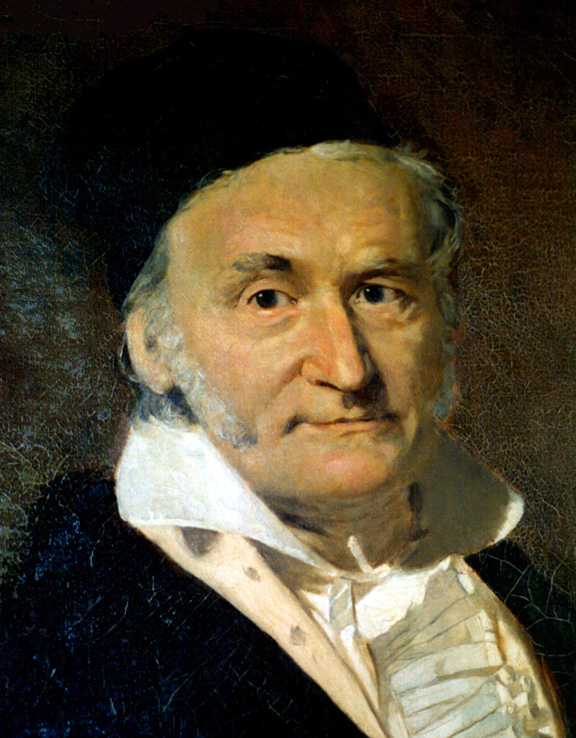
\includegraphics[width=0.8\linewidth]{img/Gauss.jpg} \\ Carl Friedrich Gauss}
		\end{minipage}
		\hfill
		\begin{minipage}[h]{0.49\linewidth}
			\center{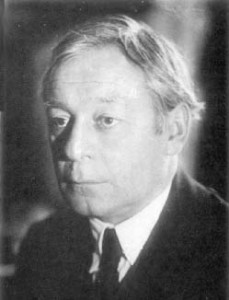
\includegraphics[width=0.8\linewidth]{img/Delone.jpg} \\ Boris Delaunay}
		\end{minipage}
	\end{figure}
\end{frame}

\begin{frame}{History}
	\begin{figure}[h]
			\center{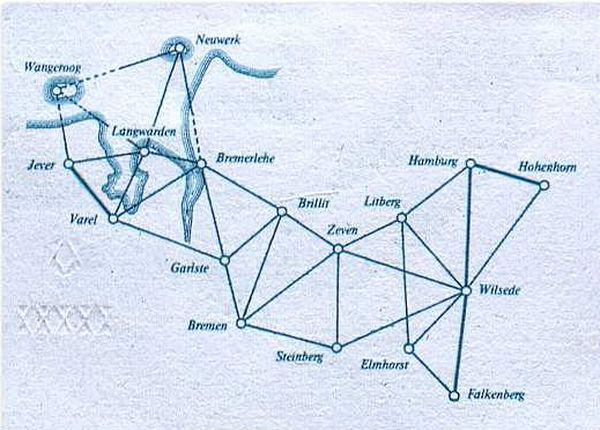
\includegraphics[width=0.8\linewidth]{img/Bremerlehe_bei_Gauss.jpg}} 
			\\ Triangulation of Kingdom of Hannover performed by Gauss (1817-1821)
	\end{figure}
\end{frame}

\begin{frame}{Application}
	\begin{itemize}
		\item \alert{Geodesy}
		\item \alert{Engineering}
		\item \alert{Image processing}
		\item \alert{3D scanning} 
	\end{itemize}
\end{frame}

\begin{frame}{Application}
	\begin{figure}[h]
			\center{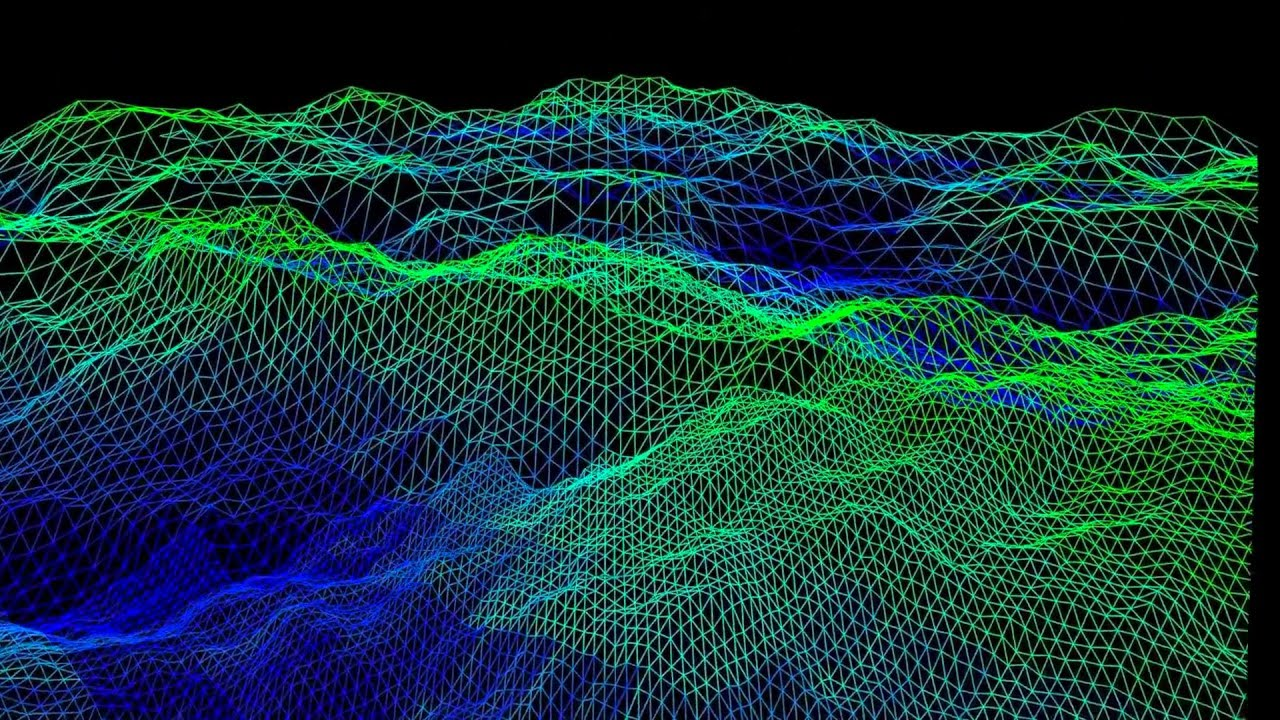
\includegraphics[width=0.8\linewidth]{img/terrain_triangulation.jpg}} 
			\\ 3D terrain triangulation
	\end{figure}
\end{frame}

\begin{frame}{Application}
	\begin{figure}[h]
			\center{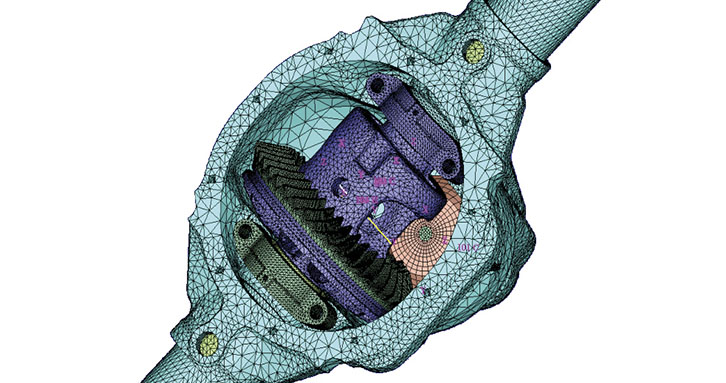
\includegraphics[width=1.\linewidth]{img/mesh.jpg}} 
			\\ 3D mesh of a vehicle differential 
	\end{figure}
\end{frame}

\begin{frame}{Application}
	\begin{figure}[h]
			\center{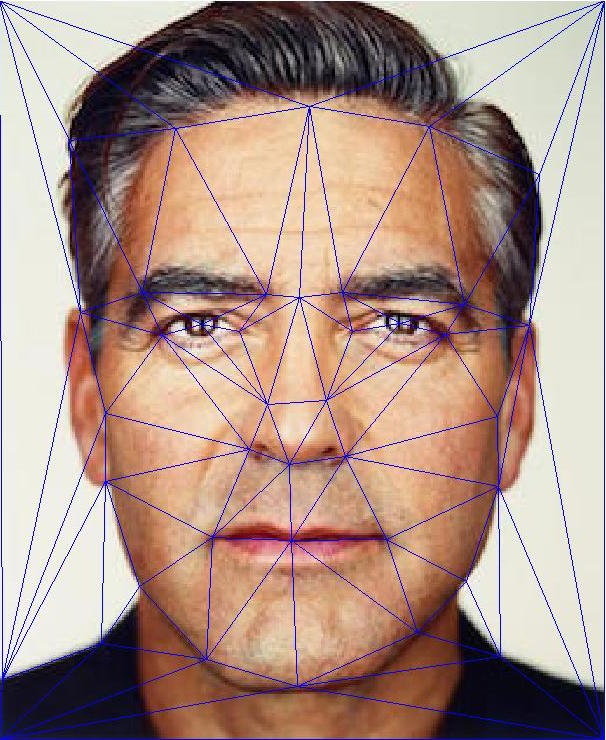
\includegraphics[width=0.5\linewidth]{img/face_triangulation.jpg}} 
			\\ Face recognition 
	\end{figure}
\end{frame}

\begin{frame}{Basic Defintion}
\begin{columns}
	\begin{column}{0.2\textwidth} 
		\begin{figure}[h]
			\center{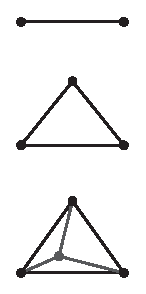
\includegraphics[width=\linewidth]{img/simplex.eps}}
		\end{figure}
	\end{column}
	\begin{column}{0.8\textwidth}
		\alert{A simplex} is a generalization of the notion of a triangle to arbitrary dimensions.		
		\bigskip
	
		Let $P=\lbrace p_1\,...,p_n\rbrace$ be a set of points in $\mathbb{R}^d$.	
		\bigskip

		$\sum_{i=1}^n \lambda_ip_i$ represents a \alert{linear combination} of points in $P$.
		\bigskip
	
		If, for $\sum_{i=1}^n \lambda_i=1$ and $\forall i, \lambda_i \geq 0$, such combination is called
		\alert{a convex hull}.
		\bigskip
	
		The convex hull of a finite number of points in $\mathbb{R}^d$ is called \alert{a polytope}.   
		\bigskip
	
		The convex hull of $k+1$ points not in an affine space of dimension $k-1$ 
		is called \alert{a simplex} or more generally \alert{a $k$-simplex}.
	\end{column}
\end{columns} 		
\end{frame}

\begin{frame}{Triangulation}
\begin{columns}
	\begin{column}{0.3\textwidth} 
		\begin{figure}[h]
			\center{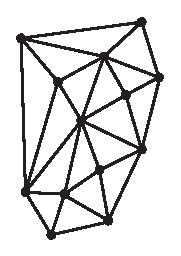
\includegraphics[width=\linewidth]{img/triangulation.eps}}
		\end{figure}
	\end{column}
	\begin{column}{0.7\textwidth} 
		Let the convex hull of $P$, denoted as \alert{$Conv(P)$}, defines a domain $\Omega$ in $\mathbb{R}^d$ 
		\bigskip
		
		The set of simplexes $\mathcal{T}_r$ is \alert{a triangulation} of $\Omega$ if
		\begin{itemize}
			\item The vertices of the elements in $ \mathcal{T}_r$ is exactly $P$.
			\item $ \Omega = \bigcup_{T \in \mathcal{T}_r}  T $.
			\item The intersection of the interior of any two elements is an empty set.
			\item The intersection of two elements in  $\mathcal{T}_r$ is either reduced to
				  the empty set or a vertex, an edge, or a face (for $d=3$ ).
		\end{itemize}
	\end{column}
\end{columns}
\end{frame}


\section{Data Structures}

\begin{frame}{Triangulation Representation}
	A triangulation can be represented by using	
	\begin{itemize}
		\item \alert{Nodes with neighbors}
		\item \alert{Double edges}
		\item \alert{Points and triangles}
		\item \alert{Points, edges and triangles}
	\end{itemize}
\end{frame}

\begin{frame}{Triangle}
	\begin{columns}
		\begin{column}{0.5\textwidth} 
			\center{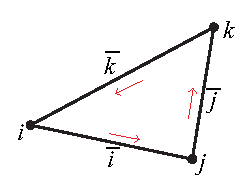
\includegraphics[width=\linewidth]{img/triangle.eps}}
		\end{column}
		\begin{column}{0.5\textwidth} 
			For storing a triangulation we will use a triangle data structure $T_{ijk}$ with
			points $i$,$j$,$k$ that have a counterclockwise orientation.
			\bigskip

			The edges $\overline{i}$, $\overline{j}$, $\overline{k}$ 
			have the same orientation. 
			\bigskip
			
			For all edges we will store adjacent triangles $T^{(i)}$, $T^{(j)}$, $T^{(k)}$.  
			\bigskip
			
			For convenience, the triangle has a local cyclic indexing.		
			
		\end{column}
	\end{columns}
\end{frame}

\begin{frame}{Triangle}
\begin{columns}
	\begin{column}{0.5\textwidth} 
		\center{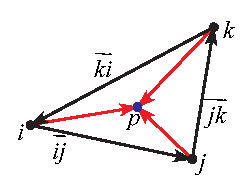
\includegraphics[width=\linewidth]{img/intriangle.eps}}
	\end{column}
	\begin{column}{0.5\textwidth} 
		A point $p$ is inside of the triangle $T_{ijk}$ iff 
		the triangle edges and $p$ makes \alert{counter-clockwise turn}, i.e.
		
		$$
			\vec{ij}\times\vec{ip} > 0,
		$$
		
		$$
			\vec{jk}\times\vec{jp} > 0,
		$$
		
		$$
			\vec{ki}\times\vec{kp} > 0.
		$$			
	\end{column}
\end{columns}	
\end{frame}

\section{Simple Algorithm}

\begin{frame}{Graham's scan} 
	\alert{Graham's algorithm} provides an efficient way for finding the convex hull of a set of points.
	\begin{itemize}
			\item \textit{Step 1} Choose a point $p_0$ with the lowest $x$ coordinate. 
							  Add $p_0$ to convex hull $H$.
			\item \textit{Step 2} Sort the remaining points $\lbrace p_1,...p_n\rbrace$ 
							  in angular order about $p_0$.
			\item \textit{Step 3} Iterate points. For each point $p_i$:
				\begin{itemize}
					\item If adding $p_i$ to $H$ results in making a "left turn", 
						  add $p_i$ to the  convex hull.
					\item If adding $p_i$ to $H$ results in making a "right turn", 
						  remove elements from $H$ until adding $p_i$ makes a 
						  left turn, then add $p_i$ to the convex hull. 	  
				\end{itemize}	
	\end{itemize}					
\end{frame}

\begin{frame}{Graham's Scan Visualization}
\center{
				\animategraphics[
						width = 0.9\linewidth ,					
						controls, loop
					]{1}{img/convex_hull_}{01}{14}
		}		
\end{frame}

\begin{frame}{Simple Triangulation Algorithm}
	A simple algorithm of a triangulation can be performed with using Graham's scan.
	\begin{itemize}
		\item \textit{Step 1} Sort $P$ in ascending $y$ coordinate order.
		\item \textit{Step 2} Add triangle $T_{012}$ to triangulation $ \mathcal{T}_r$.
		\item \textit{Step 3} Iterate points starting from $p_3$. For each point $p_i$:
			\begin{itemize}
				\item Build convex hull $H_i$ for points $p_0,...,p_i$.
				\item Compare $H_i$ with $H_{i-1}$ and find a part of $H_{i-1}$ 
					  not in $H_i$ with points $p_k,...,p_k+m$.
				\item Add triangles $T_{i j j+1}, j=\overline{k,m-1}$ to $ \mathcal{T}_r$.	    
			\end{itemize}
	\end{itemize}
\end{frame}


\begin{frame}{Visualization of a Simple Triangulation}
\center{
				\animategraphics[
						width = 0.9\linewidth ,					
						controls, loop
					]{1}{img/simple_triangulation_}{00}{09}
			}
\end{frame}

\section{Optimal Triangulation}

\begin{frame}{Non-unique triangulation}
	But which triangulation?
	\begin{figure}[h]
		\begin{minipage}[h]{0.49\linewidth}
			\center{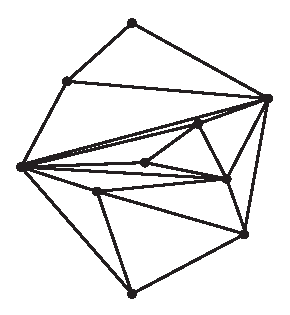
\includegraphics[width=0.8\linewidth]{img/simple_triangulation.eps} }
		\end{minipage}
		\hfill
		\begin{minipage}[h]{0.49\linewidth}
			\center{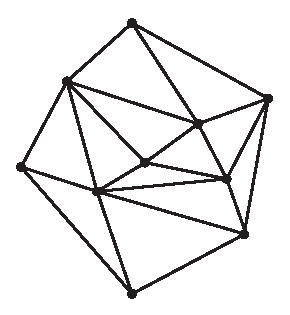
\includegraphics[width=0.8\linewidth]{img/improved_triangulation.eps}}
		\end{minipage}
	\end{figure}
\end{frame}

\begin{frame}{Angle Vector of Triangulation}
	\begin{columns}
		\begin{column}{0.4\textwidth} 
			\center{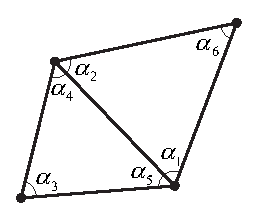
\includegraphics[width=\linewidth]{img/angle_triangulation.eps}}
		\end{column}
		\begin{column}{0.6\textwidth} 
			Let $\mathcal{T}_r$ be a triangulation of $P$ with $m$ triangles. 
			Its \alert{angle vector} is $\mathcal{A}(\mathcal{T}_r)=(\alpha_1,...,\alpha_{3m})$
			where $\alpha_1,...,\alpha_{3m}$ are the angles of $\mathcal{T}_r$ 
			sorted by increasing value.
			\bigskip
	
			Let $\mathcal{T}_r'$  another triangulation of $P$. 
			We define $\mathcal{A}(\mathcal{T}_r) > \mathcal{A}(\mathcal{T}_r')$ 
			if $\mathcal{A}(\mathcal{T}_r)$ is \alert{lexicographically} larger than
			$\mathcal{A}(\mathcal{T}_r')$.
			\bigskip
	
			$\mathcal{T}_r$ is \alert{optimal} 
			if $\mathcal{A}(\mathcal{T}_r) \geq \mathcal{A}(\mathcal{T}_r')$
			for all triangulations $\mathcal{A}(\mathcal{T}_r')$ of $P$. 		
		\end{column}
	\end{columns}
\end{frame}


\section{Delauney Triangulation}

\begin{frame}{Basic Idea. Edge Flipping}
	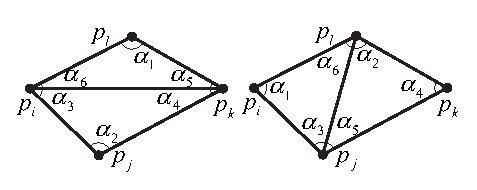
\includegraphics[width=\linewidth]{img/flip_triangle.eps}
	
	Flipping of an edge leads to changing in angle vector:
	
	$\alpha_1,...,\alpha_6$ are replaced by $\alpha_1',...,\alpha_6'$.
	\bigskip	
	
	The edge $\overline{p_ip_j}$ is \alert{illegal} 
	if $\min_{1\leq i \leq6}\alpha_i < \min_{1\leq i \leq6}\alpha_i' $ 

\end{frame}

\begin{frame}{Characteristic of Illegal Edges}
	\begin{columns}
		\begin{column}{0.6\textwidth} 
			\center{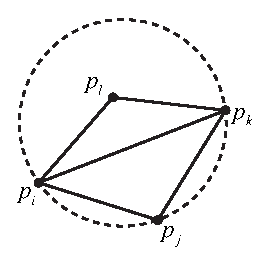
\includegraphics[width=\linewidth]{img/illegal_triangle.eps}}
		\end{column}
		\begin{column}{0.4\textwidth} 
			How do we determine if an edge is illegal?
			\bigskip
	
			The edge $\overline{p_ip_j}$ is illegal iff $\overline{p_l}$ 
			lies in the interior of the circle $C$.
		\end{column}
	\end{columns}
\end{frame}

\begin{frame}{Thales' Theorem}

	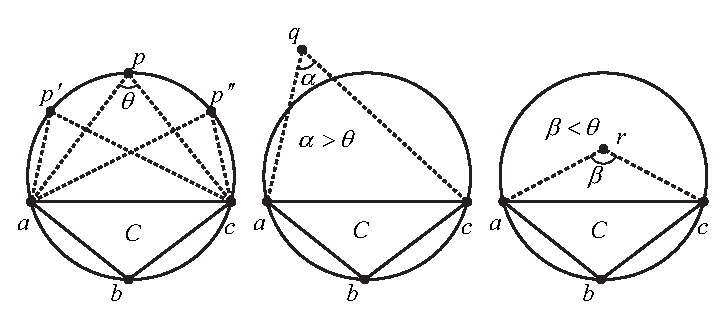
\includegraphics[width=\linewidth]{img/ThalesTheorem.eps}
	
	Let $C$ be a circle, $\overline{ab}$ is a chord of $C$, and
	$p,p',p'',q, r$ points lying on the same side of $\overline{ab}$.
	Suppose that $p,p',p'', q$ lie on $C$. Then
	$$
		\angle apc = \angle ap'c = \angle ap''c = \theta,
	$$ 
	$$
		\angle aqc = \alpha, \angle arc' = \beta,
	$$
	$$	
		\alpha < \theta < \beta
	$$
\end{frame}

\begin{frame}{Delauney triangulation}
\begin{columns}
		\begin{column}{0.4\textwidth} 
			\center{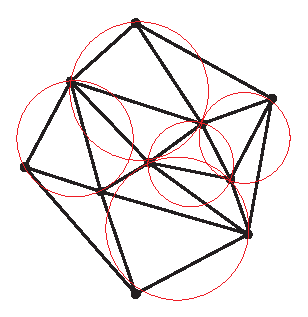
\includegraphics[width=\linewidth]{img/Delaunay.eps}}
		\end{column}
		\begin{column}{0.6\textwidth}
			A \alert{legal} triangulation is a triangulation that does not contain
			any illegal edge.
			\bigskip
	
			$\mathcal{T}_r$ is a \alert{Delaunay triangulation} of $P$  
			if the open (balls) discs circumscribed associated with its elements are empty.
			\bigskip
	
			Any angle-optimal triangulation of $P$ is a Delaunay triangulation of $P$.
			Furthermore, any Delaunay triangulation of $P$ maximizes the minimum angle
			over all triangulations of $P$.
		\end{column}
	\end{columns}
\end{frame}

\begin{frame}{Parabolic lifting}
	\begin{columns}
		\begin{column}{0.4\textwidth} 
			\center{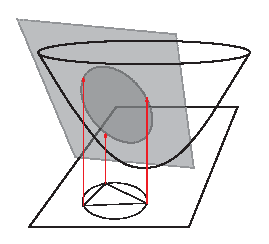
\includegraphics[width=\linewidth]{img/lifting.eps}}
		\end{column}
		\begin{column}{0.6\textwidth}
			Consider the (parabolic) \alert{lifting map}.
			For a point $p=(x,y)\in \mathbb{R}^2$ lifting $\ell(p)$ is the point			
			$$
				\ell(p) = (x,y,x^2+y^2) \in \mathbb{R}^3
			$$
			
			Let $C \subseteq \mathbb{R}^2$ be a circle of positive radius. 
			The "lifted circle" $\ell(C)$ is contained in a unique plane 
			$h_C in \mathbb{R}^3$. Moreover, a point $p \in \mathbb{R}^2$
			is strictly inside (outside) of $C$ iff $\ell(p)$ below(above) $h_C$
		\end{column}
		
	\end{columns} 

\end{frame}

\begin{frame}{Parabolic lifting}
	\begin{columns}
		\begin{column}{0.4\textwidth} 
			\center{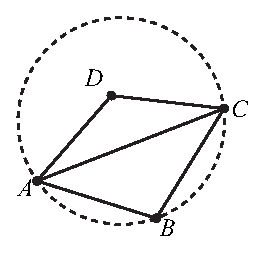
\includegraphics[width=\linewidth]{img/incircle.eps}}
		\end{column}
		\begin{column}{0.6\textwidth}
			Let $T_{ABC}$ be a triangle with vertices $A,B,C$ 
			and $D$ is a point outside $T_{ABC}$. 
			Then the condition that $D$ lies in circumscribed circle can be written as
			$$
			\begin{vmatrix}
			x_A & y_A & x_A^2 +y_A^2 & 1 \\
			x_B & y_B & x_B^2 +y_B^2 & 1 \\
			x_C & y_C & x_C^2 +y_C^2 & 1 \\
			x_D & y_D & x_D^2 +y_D^2 & 1 \\
			\end{vmatrix} 
			 >0 
			$$.
			
		\end{column}
	\end{columns} 
\end{frame}

\begin{frame}{Robust algorithm}
	
	\alert{The robust} algorithm of Delaunay triangulation based on two-pass approach. 
	
	\begin{itemize}
		\item \textit{Step 1} Build any a non-optimal triangulation.
		\item \textit{Step 2} Iterate the triangulation while it contains a pair of triangles 
							  that have an illegal edge. 
		\item \textit{Step 2} If an illegal is founded, flip it. 		
	\end{itemize}		
	

\end{frame}

\begin{frame}{Incremental algorithm}
\begin{columns}
		\begin{column}{0.4\textwidth} 
			\center{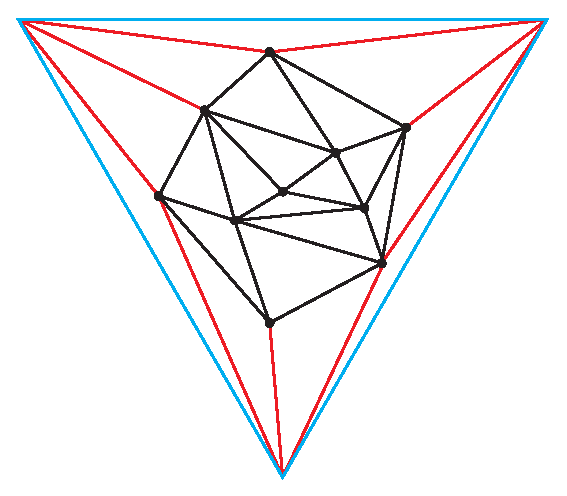
\includegraphics[width=\linewidth]{img/iterative.eps}}
		\end{column}
		\begin{column}{0.6\textwidth}
			\alert{Incremental triangulation} algorithms are based on sequential addition of points 
			to a triangulation.  
			\begin{itemize}
				\item \textit{Step 1} Build a \alert{super triangle} that contains $P$.
				\item \textit{Step 2} Add a point to the triangulation:
					\begin{itemize}
						\item Find triangle that contains the point.
						\item If the point lies on edge, divide two adjacent triangles into four parts.
						\item If the point lies in triangle interior, divide triangle into three parts.
						\item Improve triangulation.
					\end{itemize}
				\item \textit{Step 3} Remove triangles that contains the vertices of the super triangle.
			\end{itemize}
		\end{column}
		
	\end{columns} 

\end{frame}
 
\end{document}

